\subsubsection{Modelo Programa}

Este modelo conforma la base del programa que posteriormente definiremos en el \gls{dsl}. Es la base del proyecto, a partir de este \gls{metamodelo}, generaremos programas mediante un \gls{dsl} creado con \gls{xtext}. 

Este modelo representa un programa \gls{iot} en el que tenemos una serie de entradas, ya sean desde el propio \gls{gpio}, una serie de entradas remotas y acciones tanto en el propio \gls{gpio} como notificaciones remotas.

Como ejemplo, imaginemos un dispositivo \gls{iot} de lo más simple, con una sola entrada digital, utilizado para contabilizar monedas de una máquina de refrescos. Mediante el \gls{dsl} que definimos en este proyecto podríamos generar un programa para una plataforma determinada que cumpla con las siguientes características: Gestión de la interrupción \gls{gpio} asociada a dicho evento de pulso de entrada de moneda, notificación a servidor de este evento,  control de salud del propio dispositivo, etc.

El programa define una serie de \gls{gpio} pin, indicando estos con un alias, es decir, podemos asignar un nombre a una entrada, por ejemplo, \gls{led} rojo \textrightarrow pin1. Cuenta con asignación de nombres de eventos remotos, y rutas de archivos a utilizar por el programa. Un programa cuenta con una serie de estados, necesario indicar el estado principal de arranque de este y posibilitando cambiar de estado. Un ejemplo de uso real es el testeo en el arranque de los diversos indicadores \gls{led} u otras entradas/salidas, y una vez terminado, pasar a un estado de error en caso de fallo, y en caso de funcionamiento normal, pasar al estado del programa principal.


En la figura \ref{fig:modelo_iot_programa_classes} podemos visualizar en formato diagrama de clases \gls{uml} el modelo \textit{Program}.

\begin{figure}
	\centering
    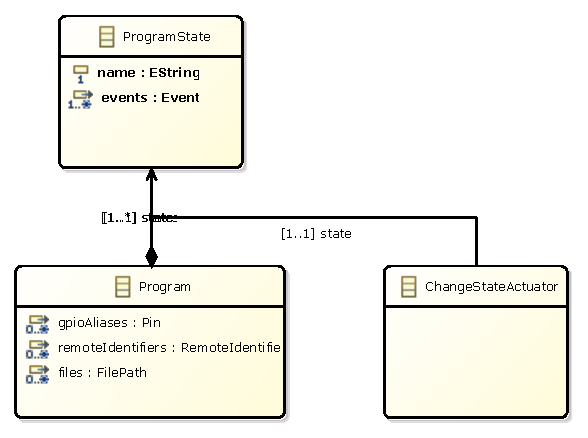
\includegraphics[height=0.3\textheight]{images/models/programs_class_diagram.pdf}
    \captionmodeloclase{Programa IOT}
    \label{fig:modelo_iot_programa_classes}
\end{figure}

\clearpage
